\section{Markt und Differenzierung}
Um zu sehen, ob unsere Geschäftsidee Anschluss im Markt finden würde, wurde zuerst das Marktpotential berechnet. 

%Bild marktanalyse einfügen
\begin{figure}[H]
	\centering
	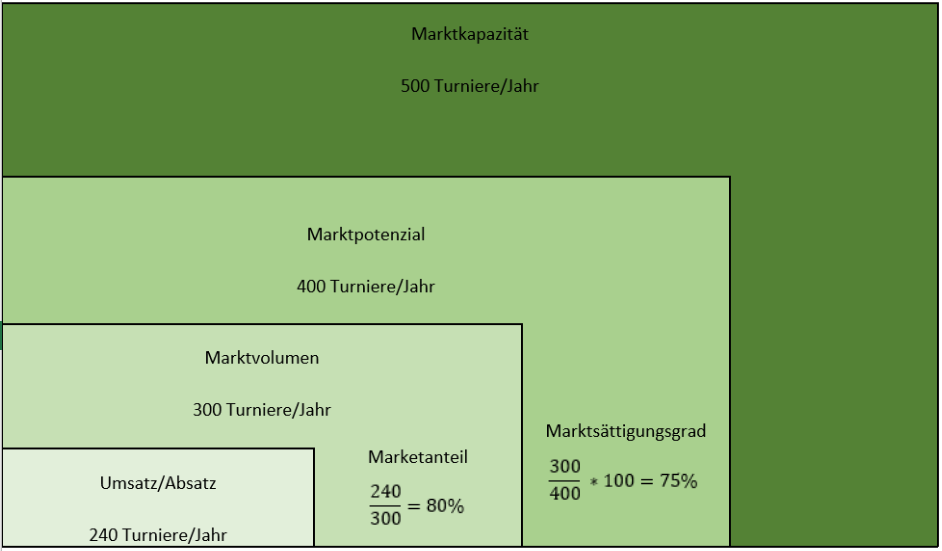
\includegraphics[width=0.85\linewidth]{images/marktanalyse.PNG}
	\caption{Marktanalyse}
	\label{fig:marktanalyse}
\end{figure}

Wie man sieht, sollte es auf dem Markt noch Platz haben für unser Produkt.
Die Zahlen gelten nicht für das erste Jahr, sondern sind gross gerechnet, nach ca. 5 Jahren.
In dieser Zeit sollte sich unser Produkt herumgesprochen und verbreitet haben.
Wir rechnen damit, dass wir von Österreich her aus dem Taekwondo starten und unseren Einflussbereich Jahr für Jahr vergrössern. So sollte die App nach 5 Jahren europaweit bekannt und genutzt werden.
Ausserdem wollen wir noch neue Sportarten hinzunehmen, beziehungsweise neue Bewertungsmöglichkeiten in unserer App anbieten.
Das könnten z.B. Eiskunstlaufen, Geräteturnen und Gymnastik sein.
\\
Unsere Lösung zeichnet sich dadurch aus, dass sie sehr stabil und flexibel ist.
Da sie plattformunabhängig ist, braucht man kein spezielles Gerät, sondern jeder Bewerter kann sein eigenes Handy dafür benutzen.
So bleibt es unkompliziert und man kann sich die Mietkosten für die Hardware sparen.
Falls es jedoch gewünscht ist, kann man diese auch direkt bei uns mitmieten.
Dank verschiedenen Abos und dem App ist unser System auch sehr kostengünstig.
Falls man sich trotz der einfachen Bedienung noch unsicher fühlt, bieten wir eine Supporthotline an und verschiedene Schulungen.
Auch die Coronapandemie stellt für unsere Software kein Hindernis dar, denn es ist als Onlinesystem ausgeführt und so auch von jedem Zuhause aus bedienbar.
\\\\
Damit möglichst viele von unserem Produkt erfahren, wollen wir unsere Software direkt den Taekwondo-Vereinen und den Veranstaltern von solchen Turnieren vorstellen.
Da wir selbst jemanden haben aus einem solchen Verein, wollen wir die Software zuerst vor allem durch Mundpropaganda bekannt machen.
Eventuell auch die Flyer oder Werbung direkt an die Vereine schicken oder an Turnieren verteilen.
So sollte sich unsere Lösung schnell herumsprechen und neue Kunden anlocken.
Bei neuen Sportarten würden wir ähnlich vorgehen und uns gezielt Leute suchen, welche schon eine Weile diese Sportart ausüben und sich darin auskennen.
So kann die Bewertungsapp auf die spezifische Sportart angepasst werden.

\subsection{Markt}
Eine genaue Marktanalyse ist schwierig. Um genaue Informationen zu erhalten müsste man die einzelnen Kreis- und Landesverbände kontaktieren. Dies zeigt jedoch bereits, dass es bisher keine einheitliche und weithin bekannte Lösung gibt. Es existieren bisher Tools, um genaue Videoanalysen in Zeitlupe zu machen, wie sie beispielsweise in der Gymnastik eingesetzt werden. Weiter gibt es Software, welche es erlaubt, Turnierbewertungen zu verwalten. Jedoch steht keine Onlinelösung zur Verfügung noch stellen sie Hardware zur Verfügung.\\  
Ausserdem ist davon auszugehen, dass bisherige Systeme sich auf eine Sportart beschränken. Unser System lässt sich im Taekwondo, Eiskunstlauf, Gymnastik wie auch Geräteturnen einsetzen und soll künftig auch auf weitere Sportarten ausgeweitet werden.  

\subsection{Unfairer Vorteil}
Wie sich im vergangenen Jahr gezeigt hat, können unvorhergesehene Ereignisse auftreten, welche Turnierveranstalter*innen zwingen, mit neuen Ideen aufzuwarten. Unser System kann sowohl für reguläre Turniere eingesetzt werden wie auch für Online-Turniere, wie sie in Pandemiezeiten stattfinden können. Dieses Feature ist ein entscheidender Vorteil gegenüber anderen Systemen.\\
Des Weiteren wird unser System mit fundiertem Wissen im technischen wie auch im sportlichen Bereich entwickelt. Die sportlichen Kenntnisse beschränken sich im Moment auf Taekwondo. Es ist anzunehmen, dass dies als Grundlage ausreichend ist und für die Sportarten Eiskunstlauf, Gymnastik und Geräteturnen nur geringfügige Modifikationen notwendig sind.